% How one commercial render is split into single operations, drawn from results/research/retouch_unified_20260929/decompose.py
% on the Tencent pair FFHQ 60002 (render applies whitening, smoothing, face lifting and eye enlarging at once).
% Tiles: make_tiles_method.py (method_vendor_*, method_comp_*) and make_tiles_engine.py (engine_*; its check: the four
% components are bit-identical to decompose.decompose, reconstruction 108.1 dB). Build: make_fig_engine.sh.
% Same visual language as fig_method (panel, chip title, tiles 2.2 cm wide, class-coloured tile borders).
% Top row: geometry (flow f split by the eye mask). Bottom row: photometry (residual P split by a Gaussian low-pass).
\documentclass[border=0pt]{standalone}
\usepackage{fontspec}
\setmainfont{Liberation Sans}
\usepackage{tikz}
\usetikzlibrary{arrows.meta,positioning,calc}
\definecolor{nn}{HTML}{0F4D92}
\definecolor{ink}{HTML}{222222}
\definecolor{muted}{HTML}{5E6670}
\definecolor{fp}{HTML}{26A6DC}
\definecolor{rl}{HTML}{009E73}
\definecolor{bt}{HTML}{C98A00}
\definecolor{panel}{HTML}{F4F6F9}
\definecolor{pline}{HTML}{C9D1DB}
\newcommand{\vi}[1]{\textit{#1}}
\newcommand{\me}{\vi{m}\textsubscript{e}}
\begin{document}
\fontsize{9}{10.8}\selectfont
\hyphenpenalty=10000 \exhyphenpenalty=10000
\begin{tikzpicture}[
  x=1cm, y=1cm, text=ink,
  >={Latex[length=1.9mm,width=1.6mm]},
  ar/.style={->, line width=0.7pt, draw=ink},
  ln/.style={line width=0.7pt, draw=ink},
  tile/.style={inner sep=0pt, outer sep=0pt, anchor=south west},
  lab/.style={align=center, inner sep=0pt},
  chip/.style={fill=nn, text=white, font=\fontsize{10}{12}\selectfont\bfseries, rounded corners=6pt, inner xsep=7pt, inner ysep=3pt},
  tag/.style={draw=nn, text=nn, font=\fontsize{9}{10}\selectfont\bfseries, rounded corners=5pt, inner xsep=5pt, inner ysep=2pt, fill=white},
]
\def\tw{2.2cm}
\def\yt{5.1}    % top row (tiles 2.2 x 2.64 cm)
\def\yb{0.95}   % bottom row
\def\cA{0.2} \def\cB{3.1} \def\cC{6.0} \def\cD{8.9} \def\cE{11.8}
% ---------------------------------------------------------------- panel and title
\draw[draw=pline, fill=panel, rounded corners=6pt, line width=0.6pt] (0,0) rectangle (14.66,9.15);
\node[chip, anchor=west] at (0.15,9.15) {One commercial render, split into single operations with exact footprints};

% ---------------------------------------------------------------- inputs
\node[tile] (O) at (\cA,\yt) {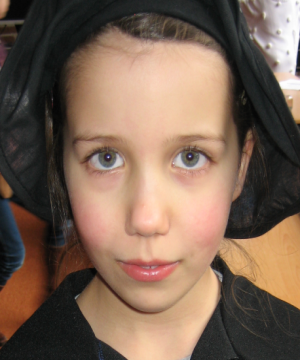
\includegraphics[width=\tw]{figs/method_vendor_O.png}};
\node[tile] (R) at (\cA,\yb) {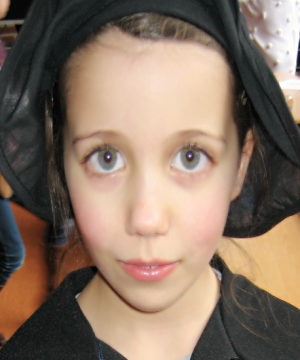
\includegraphics[width=\tw]{figs/method_vendor_R.png}};
\draw[rl, line width=1.4pt, rounded corners=2pt] (O.south west) rectangle (O.north east);
\draw[bt, line width=1.4pt, rounded corners=2pt] (R.south west) rectangle (R.north east);
\node[lab, anchor=south] at ($(O.north)+(0,0.1)$) {original \vi{O}};
\node[lab, anchor=north] at ($(R.south)+(0,-0.1)$) {render \vi{R}};

% ---------------------------------------------------------------- geometry
\node[tile] (F) at (\cB,\yt) {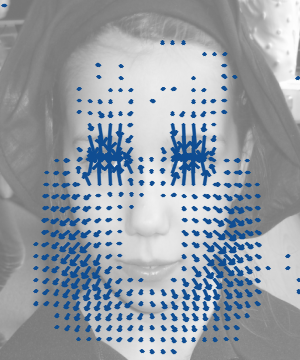
\includegraphics[width=\tw]{figs/engine_flow.png}};
\node[lab, anchor=south] at ($(F.north)+(0,0.1)$) {optical flow \vi{f}\\\vi{O}(\vi{x}+\vi{f}) ≈ \vi{R}(\vi{x})};
\node[tile] (E) at (\cC,\yt) {
\includegraphics[width=\tw]{figs/engine_eyes.png}};
\node[lab, anchor=south] at ($(E.north)+(0,0.1)$) {eye mask \me\\from landmarks};
\node[tile] (Ce) at (\cD,\yt) {
\includegraphics[width=\tw]{figs/method_comp_eye.png}};
\node[tile] (Cc) at (\cE,\yt) {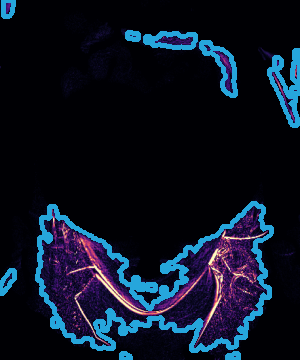
\includegraphics[width=\tw]{figs/method_comp_contour.png}};
\draw[bt, line width=1.4pt, rounded corners=2pt] (Ce.south west) rectangle (Ce.north east);
\draw[bt, line width=1.4pt, rounded corners=2pt] (Cc.south west) rectangle (Cc.north east);
\node[lab, anchor=south] at ($(Ce.north)+(0,0.1)$) {\textbf{eye}\\\vi{O}(\vi{x} + \me\vi{f})};
\node[lab, anchor=south] at ($(Cc.north)+(0,0.1)$) {\textbf{contour}\\\vi{O}(\vi{x} + (1−\me)\vi{f})};
\draw[ar] (O.east) -- (F.west);
\draw[ar] (R.north east) -- (F.south west);
\draw[ar] (F.east) -- (E.west);
\draw[ar] (E.east) -- (Ce.west);
\draw[ln] ($(E.east)!0.5!(Ce.west)$) |- (12.9,4.82);
\draw[ar] (12.9,4.82) -- (Cc.south);

% ---------------------------------------------------------------- photometry
\node[tile] (P) at (\cB,\yb) {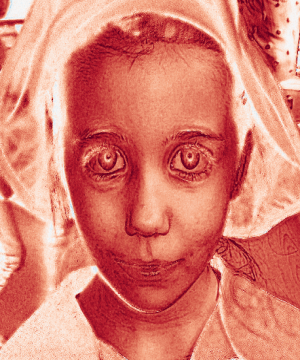
\includegraphics[width=\tw]{figs/engine_resid.png}};
\node[lab, anchor=north] at ($(P.south)+(0,-0.1)$) {residual\\\vi{P} = \vi{R} − \vi{O}(\vi{x}+\vi{f})};
\node[tile] (Ct) at (\cD,\yb) {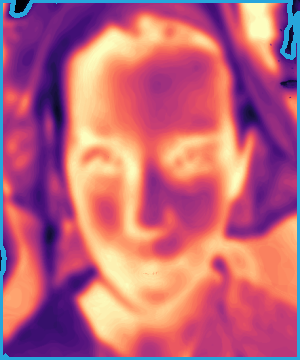
\includegraphics[width=\tw]{figs/method_comp_tone.png}};
\node[tile] (Cx) at (\cE,\yb) {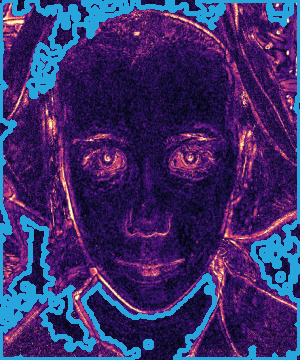
\includegraphics[width=\tw]{figs/method_comp_texture.png}};
\draw[bt, line width=1.4pt, rounded corners=2pt] (Ct.south west) rectangle (Ct.north east);
\draw[bt, line width=1.4pt, rounded corners=2pt] (Cx.south west) rectangle (Cx.north east);
\node[lab, anchor=north] at ($(Ct.south)+(0,-0.1)$) {\textbf{tone}\\\vi{O} + low(\vi{P})};
\node[lab, anchor=north] at ($(Cx.south)+(0,-0.1)$) {\textbf{texture}\\\vi{O} + high(\vi{P})};
\draw[ar] (R.east) -- (P.west);
\draw[ar] (F.south) -- (P.north);
\draw[ar] (P.east) -- node[above=3pt, lab, xshift=-0.2cm] {Gaussian low-pass\\σ = 6 px} (Ct.west);
\draw[ln] (8.6,2.27) |- (12.9,3.88);
\draw[ar] (12.9,3.88) -- (Cx.north);
\node[lab, anchor=south east] at (8.5,3.3) {high = \vi{P} − low};

% ---------------------------------------------------------------- side card: checks and yield (full text width 18.13 cm)
\draw[draw=pline, fill=panel, rounded corners=6pt, line width=0.6pt] (14.96,0) rectangle (18.13,9.15);
\node[fill=ink!80, text=white, font=\fontsize{10}{12}\selectfont\bfseries, rounded corners=6pt, inner xsep=7pt, inner ysep=3pt,
      anchor=west] at (15.11,9.15) {What it gives};
\node[draw=pline, fill=white, rounded corners=3pt, line width=0.5pt, anchor=north west, text width=2.62cm, align=left,
      inner sep=4pt] (k1) at (15.15,8.55)
  {\textbf{Exact}\\[1pt]\vi{O}(\vi{x}+\vi{f}) + \vi{P} = \vi{R} by construction;\\[1pt]
   {\fontsize{15}{17}\selectfont\bfseries 108 dB}\\ reconstruction};
\node[draw=pline, fill=white, rounded corners=3pt, line width=0.5pt, anchor=north west, text width=2.62cm, align=left,
      inner sep=4pt] (k2) at ($(k1.south west)+(0,-0.22)$)
  {\textbf{A footprint each}\\[1pt]\vi{M} = |\vi{C} − \vi{O}| > 6 of 255, dilated (\textcolor{fp}{\textbf{cyan}})};
\node[draw=pline, fill=white, rounded corners=3pt, line width=0.5pt, anchor=north west, text width=2.62cm, align=left,
      inner sep=4pt] (k3) at ($(k2.south west)+(0,-0.22)$)
  {\textbf{Yield}\\[1pt]{\fontsize{15}{17}\selectfont\bfseries 50,112}\\ single-operation items from 18,734 renders (Tencent, Megvii); Alibaba is never decomposed};
\end{tikzpicture}
\end{document}
